\section{Organizando nossas editathonas}

A fim de estudar a dificuldade de entrada de novos/as usuários/as \textit{in loco}, em nossa abordagem de pesquisa ``de fora para dentro'', resolvemos organizar nossas próprias editatonas como atividades de campo. Podendo assim observar problemas encontrados pelos/as participantes, e mapear com eles/as os mecanismos de governança da Wikipédia que se apresentam como barreiras, muitas vezes intransponíveis, deixando novatos/as bem intencionados/as sem saber como prosseguir.

Com isto, partindo das observações feitas \textit{in loco} nas editatonas, regressamos a bancada de ciência de dados de nosso laboratório. Nela andamos colados ao banco de dados, realizando inferências nos dados abertos da Wikipédia. Investigamos padrões, elementos e comportamentos da governança da comunidade que interagiram com nossos participantes durante e após as editatonas.

\subsection{Por que resolvemos fazer editatonas?}

A metodologia adotada de realizar editatonas foi validada como pertinente logo no início da pesquisa em 2017, com a realização de uma atividade em sala de aula com a turma de pós-graduação da disciplina ``\textit{Estudos CTS (Ciências-Tecnologias-Sociedades): aproximações brasileiras e latino-americanas}'', ministrada no Programa de Engenharia de Sistemas e Computação da COPPE/UFRJ, no 2º período de 2017. Atividade esta que teve seus resultados retratados no trabalho ``\textit{Práticas de escrita biográfica na Wikipédia em português em turmas de pós-graduação}'', apresentado no VII Simpósio Nacional de Ciência, Tecnologia e Sociedade (Esocite.BR), também em 2017 (\cite{andrade_historias_2017}).

A editatona foi realizada durante uma aula em que o professor não poderia estar presente, e os/as estudantes deveriam se auto organizar e autogerir para realizar alguma atividade. Inicialmente o grupo imaginava que iria trabalhar no CTS Brasil Blog, site idealizado para escoar produções feitas ao longo do curso. Mas, no momento do encontro, percebeu-se que a produção deste já tinha seu fluxo de trabalho remoto bem definido, e que as horas que teríamos juntos presencialmente poderiam ser melhor aproveitadas de outra forma.

Assim, com a decisão de realizarmos uma editatona, fiz uma apresentação sobre o funcionamento da Wikipédia e suas políticas editoriais. Propus então para o grupo que o escopo da atividade fosse o desenvolvimento de verbetes biográficos sobre os autores CTS que estávamos estudando\footnote{No capítulo 4 detalhamos as práticas de escrita biográfica que já estavam ocorrendo durante a disciplina.}. O grupo então debateu sobre quais verbetes editar, e entendendo que existia um artigo que precedia os biográficos em importância para divulgação do tema CTS, definiu que seria feita uma força tarefa para melhorar apenas um verbete: ``\textit{Estudos de ciência, tecnologia e sociedade}''. Os 13 presentes então se dividiram em grupos, responsáveis por criar/melhorar diferentes seções do verbete em paralelo, que somadas comporiam a nova versão do verbete ao final da aula.

Antes da atividade, o verbete contava com 3.989 bytes\footnote{Unidade de medida utilizada pela comunidade para medir o tamanho de revisões e verbetes.}, com uma breve introdução e uma seção textual intitulada ``Ensino'', seguida por seções de ``Bibliografia'' e ``Ligações externas''. Três horas depois, o texto já apresentava 23.570 bytes, sendo 20.281 bytes adicionados pela turma e 18 bytes adicionados pelo usuário FSogumo, que não era aluno do curso e adicionou, durante a atividade, o \textit{template} de geração automática de referências ao verbete, que agora contava com dez seções textuais diferentes.

Sabendo da dificuldade tão relatada de conteúdos criados em salas de aula persistirem por um longo período de tempo na Wikipédia (\cite{marques_trabalhando_2012}), (\cite{carver_assigning_2012}), (\cite{archuby_experiencias_2018}), (\cite{soler-adillon_wikipedia_2018}), voltamos então ao verbete ``\textit{Estudos de ciência, tecnologia e sociedade}'' um mês depois da realização da atividade, para pesquisar o que teria acontecido com as edições de nossos/as editores/as.

Encontramos mais três edições feitas por alunos da turma no verbete após a atividade, adicionando mais 10.551 bytes, e percebemos uma situação que contradiz toda a literatura sobre editatonas: nenhuma edição de nossa turma havia sido revertida, e todo o conteúdo criado por nossos/as novos/as editores/as continuava no ar. Este fato é ainda mais surpreende pois em nossa atividade os/as estudantes foram estimulados/as a editar diretamente a Wikipédia, sem realizar uso prévio das páginas de testes, o que diminuiria ainda mais as chances de sobrevivência de seus conteúdos (\cite{marques_trabalhando_2012}).

Perante tão distinta situação, resolvemos então investigar o que havia acontecido de especial em nossa editatona, e enredamos a ferramenta \textit{Objective Revision Evaluation Service} (ORES)\footnote{Em português Sistema Objetivo de Avaliação de Revisões.}, para analisar todas as edições feitas durante a atividade.

O ORES é uma ferramenta de inteligência artificial que avalia edições (também chamadas pelos/as usuários/as de revisões) feitas nas Wikipédias. Solicitamos aqui de nossos/as leitores/as a gentileza de aceitar o ORES como uma caixa-preta (assim como ela é aceita pelos/as editores/as e reversores/as das Wikipédias)\footnote{Na verdade no uso cotidiano da enciclopédia o ORES faz parte das redes que sustentam outras caixas pretas, enquanto ele fica invisível fazendo suas avaliações no backend e seu nome permanece desconhecido para a maior parte da comunidade.}, e tomemos suas saídas como avaliações confiáveis sobre as edições apreciadas. Para cada edição, o ORES nos indica probabilidades de ser danosa, feita em boa fé e de ser revertida (``apagada'').

\begin{center}
\begin{table}
\begin{tabular}{ |c|c|c|c| } 
 \hline
\textbf{Id da Edição} & \textbf{Não danosa} & \textbf{Feita em boa fé} & \textbf{Deve ser revertida} \\
\hline
49529742 & 76\% & 87\% & 65\% \\
\hline
49529756 & 76\% & 90\% & 33\% \\
\hline
49529775 & 52\% & 59\% & 71\% \\
\hline
49529792 & 36\% & 35\% & 76\% \\
\hline
49529803 & 80\% & 84\% & 58\% \\
\hline
49529830 & 58\% & 61\% & 73\% \\
\hline
49529836 & 24\% & 34\% & 76\% \\
\hline
49529856 & 42\% & 56\% & 69\% \\
\hline
49531419 & 54\% & 63\% & 72\% \\
\hline
\textbf{49531652} & \textbf{98\%} & \textbf{99\%} & \textbf{04\%} \\
\hline
49781518 & 91\% & 96\% & 12\% \\
\hline
49785059 & 86\% & 88\% & 41\% \\
\hline
49802969 & 67\% & 88\% & 32\% \\
\hline
Média & 64\% & 72\% & 52\% \\
 \hline
\end{tabular}
\caption{Avaliação feita pelo ORES de todas as edições feitas na atividade, com a edição do coordenador destacada em negrito.}
\label{table:avaliacao-ores}
\end{table}
\end{center}

A tabela \ref{table:avaliacao-ores} exibe a avaliação do ORES para todas as edições feitas no contexto de nossa editatona, começando da mais recente e descendo cronologicamente. Observando a tabela podemos notar que a maioria de nossas edições foram vistas pelo sistema tanto feitas em boa fé como não danosas, mas apresentavam percentual alto de chances de serem revertidas.

Não por acaso, esse é exatamente o perfil de edição que organizadores de editatonas relatam vivenciar. Seus/suas colegas estão editando em boa fé e realizando alterações que não são danosas para a enciclopédia, mas a falta de um determinado padrão de escrita, esperado pela comunidade, faz com que as edições sejam revertidas.

Ao observarmos atentamente a tabela criada pelo ORES uma edição nos salta aos olhos. A edição com id \textbf{49531652} apresenta 98\% de chances de não ser danosa, 99\% de ser feita em boa fé e apenas 4\% de chances de ser revertida. Ao clicar no detalhamento desta edição, podemos ver que ela havia sido feita pelo usuário experiente que coordenava a atividade (eu), e, nesta edição de 839 \textit{bytes}, todos os conteúdos criados nas edições anteriores eram revisados, sendo colocados no formato wikipédico, com ligações internas e referências no padrão wiki.

Esta edição específica, além de auxiliar a manter na enciclopédia os conteúdos que, segundo o ORES, tinham grandes chances de serem revertidos, estrutura o verbete e ajuda os próximos editores a criarem conteúdos mais ``aceitáveis'' para enciclopédia. As três edições seguintes a essa, feitas por alunos da turma, observam suas chances de serem revertidas caírem drasticamente. Antes da edição do coordenador da atividade, as edições dos novatos apresentavam em média 65,88\% de chances de serem revertidas. Já as realizadas por esse mesmo recorte de usuários/as posteriormente apresentam uma enorme queda nesse valor, para apenas 28,33\%.

Percebemos, então, a importância do coordenador da atividade não ser um mero tutor que orienta os participantes e apresenta dicas de edição. Sua participação ativa na escrita coletiva dos mesmos verbetes que os/as editores/as novatos/as estiverem trabalhando pode auxiliar a manter as edições destes/as no ar, aumentando o sucesso da atividade tanto na satisfação dos participantes, como na disponibilização de mais conteúdos livres a longo prazo.

Após a alta frequência de edições feitas pela turma em agosto e setembro de 2017, a página ``\textit{Estudos de ciência, tecnologia e sociedade}'' voltou a ser pouco editada. Nos dois anos seguintes, até o final de 2019, foram feitas apenas duas contribuições com adição substancial de conteúdo, que não dialogaram com o conteúdo criado pela turma, mas criaram uma seção sobre o ``movimento CTSA (Ciência, Tecnologia, Sociedade e Ambiente)''. Essas edições adicionaram 1415 bytes ao verbete, que permaneceram no ar não revisados nem contestados até o início de 2020.

Esse baixo volume de revisões no verbete mostra a importância das editatonas para não apenas apresentar o funcionamento da Wikipédia buscando engajar novos/as editores/as, como também para produzir conteúdos em assuntos que não sejam muito populares entre os/as editores/as habituais. Apesar de suas mais de 200 mil edições por mês, a Wikipédia tende a concentrar seu maior volume de edições em tópicos como política, esportes ou televisão.

\begin{center}
\begin{table}
\begin{tabular}{ |c|c| } 
 \hline
\textbf{Verbete} & \textbf{Edições em 2019} \\ 
\hline
Big Brother Brasil 19 & 581 \\ 
\hline
Governo Jair Bolsonaro & 357 \\ 
\hline
Copa São Paulo de Futebol Júnior de 2019 & 265 \\ 
\hline
Rompimento de barragem em Brumadinho & 247 \\ 
\hline
Primeira Liga de 2018–19 & 217 \\ 
\hline
Copa da Ásia de 2019 & 197 \\ 
\hline
Campeonato Mundial de Handebol Masculino de 2019 & 182 \\ 
\hline
Lista de participantes do Big Brother Brasil & 173 \\ 
\hline
Verão 90 & 168 \\ 
\hline
Temporada do Sport Club Corinthians Paulista de 2019 & 163 \\ 
 \hline
\end{tabular}
\caption{Lista de verbetes mais editados em 2019 na Wikipédia em português.}
\label{table:verbetes-mais-editados-2019}
\end{table}
\end{center}

Assim, conteúdos criados em editatonas que tenham como temática assuntos não midiáticos tendem a não receber muitas colaborações posteriores, e a produção gerada na atividade tenderá a se estabilizar como o conteúdo que futuros leitores terão acesso em suas pesquisas. Cabe dar bastante ênfase aqui ao fato de que, ao contrários de trabalhos científicos, que ``\textit{a maioria nunca é lida por ninguém}'' (\cite[p.59]{latour_ciencia_1987}), os artigos criados na Wikipédia tem uma grande audiência. E, quanto mais conteúdos tenha um verbete, mais facilmente ele será encontrado por robôs e indexado por mecanismos de busca, fazendo com que ainda mais leitores encontrem o texto.

Com isso, quando uma editatona expande um verbete, além de estar melhorando a qualidade daquele conteúdo para a audiência esperada, ela está também aumentando o público que terá acesso àquele verbete.

\begin{figure}[H]
    \centering
    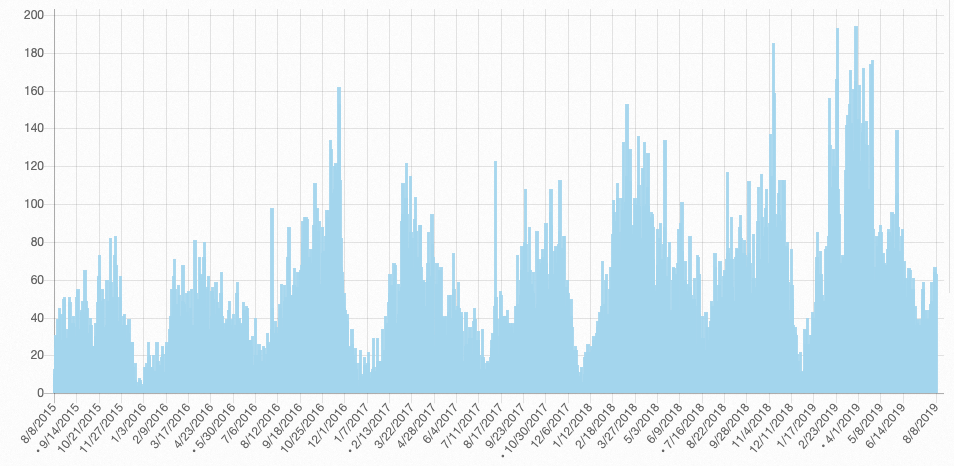
\includegraphics[width=1\textwidth]{Images/acessos-estudos-cts.png}
    \caption{Acessos ao verbete trabalhado dois anos antes e dois anos depois da atividade.}
    \label{fig:acessos-estudos-cts}
\end{figure}

Na figura \ref{fig:acessos-estudos-cts} observamos os acessos ao verbete ``\textit{Estudos de ciência, tecnologia e sociedade}'' entre 8 de agosto de 2015 e 8 de agosto de 2019, exatamente dois anos antes e dois anos depois da editatona. Diferente do trabalho apresentado em 2017 (\cite{andrade_historias_2017}), que observara dois meses antes e dois meses depois da atividade, optamos por esse recorte maior de tempo para dar conta da sazonalidade observada nos acessos ao verbete ao longo do ano, que parece ser bastante influenciada pelo calendário escolar anual.

Compreendido então o recorde, observamos que, nos dois anos anteriores à editatona, o verbete apresentava uma audiência média de 38 acessos por dia. Nos dois anos seguintes, esse número cresce 55,26\%, para 59 acessos diários.

Em valores absolutos, e considerando que o verbete manteria um volume estável de visitas com seu conteúdo anterior\footnote{Consideração benevolente, pois entre 2016 e 2019 os acessos à Wikipédia em português como um todo caíram 1,5\%, como pode ser visto em https://stats.wikimedia.org/\#/pt.wikipedia.org/reading/total-page-views/normal|bar|2016-01-01~2020-01-01|~total|monthly , acessada em 19 de março de 2020.}, isso significa que a editatona de 3 horas, com 13 participantes, proporcionou em dois anos 15.330 leituras a mais sobre ``Estudos de ciência, tecnologia e sociedade'' em português.

Perante o volume de acessos da Wikipédia, aproximadamente 13 milhões por dia somente em português, essas 15 mil leituras em dois anos podem parecer poucos relevantes. Mas, dentro de seu nicho específico de um assunto não muito midiático como ``Estudos de ciência, tecnologia e sociedade'', esse número significa que, no mundo real, 15 mil pessoas que antes não teriam encontrado esse conteúdo em português sobre o tema agora o terão, e com encontrando um texto enciclopédico com maior abrangência e mais referências do que eram apresentadas antes da editatona.

A título de comparação, podemos olhar para os números de outra atividade desenvolvida pela mesma turma: o ``CTS Brasil Blog''\footnote{Disponível em https://ctsbrasilblog.wordpress.com/ .}. Ao longo de todo o curso, os/as estudantes criaram conteúdos e os publicaram nesta página, dedicada especialmente a ``\textit{circular vídeos, resenhas, entrevistas, manifestos e o que mais sair das digestões feitas durante a disciplina}'' (\cite{cts_brasil_blog}). Ao final do curso, o site contava com 17 publicações, feitas por 10 autores/as diferentes.

No ano de sua criação o blog teve seu pico de acessos, muito provavelmente ocasionado pelas visitas dos/as próprios/as estudantes-autores, com 526 visitas. No ano seguinte, este número cai para 215 e, em 2019, o blog encerra o ano com 149 visualizações. Enquanto o volume de acessos inicial pode ser explicado pelos autores acessando o site durante a disciplina, pois só nos dois primeiros meses de vida o \textit{site} recebeu 482 visualizações, os meses seguintes de novembro e dezembro somados totalizam 44 visitas. Podemos então considerar que em outubro de 2017 o blog é estabilizado por seus/suas autores/as, que param de publicar após o término da disciplina, e que os acessos que acontecem a partir daí seriam feitos por leitores/as alheios ao curso. Assim, considerando todos os acessos dos dois últimos meses de 2017, e os anos inteiros de 2018 e 2019, no que podemos considerar leituras orgânicas\footnote{Em mídias sociais, esse é o termo utilizado para acessos feitos sem pagamento de divulgação, por usuários que encontram o site através de links externos ou buscadores.} do conteúdo, temos um volume de 408 visualizações, em uma média de 0.51 visitas por dia.

\begin{figure}[H]
    \centering
    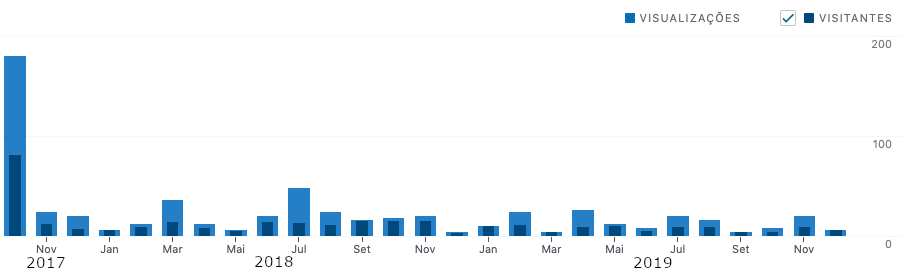
\includegraphics[width=1\textwidth]{Images/acessos-cts-brasil.png}
    \caption{Acessos ao CTS Brasil Blog por mês.}
    \label{fig:acessos-cts-brasil}
\end{figure}

Essa iniciativa do CTS Brasil Blog é claramente um caso de sucesso de divulgação científica, que continua no ar até hoje apresentando para leitores lusófonos, e em grande maioria (89,3\%, como pode ser visto na figura \ref{fig:acessos-geo-cts-brasil}) do Brasil, conteúdos sobre os Estudos de Ciências-Tecnologias-Sociedades, que outrora ficariam restritos às salas de aula de pós-graduação. Mas, seu relevante volume de acessos parece pequeno se comparado às mais de 15 mil visitas que receberam os conteúdos criados na editatona realizada pela mesma turma.\footnote{É importante destacar que o blog aceitava diferentes tipos de conteúdos, e não apenas textos enciclopédicos. Aqui comparamos seus acessos não para medir qual atividade teve maior sucesso, mas apenas para colocar o alcance da atividade realizada na Wikipédia em perspectiva.}

\begin{figure}[H]
    \centering
    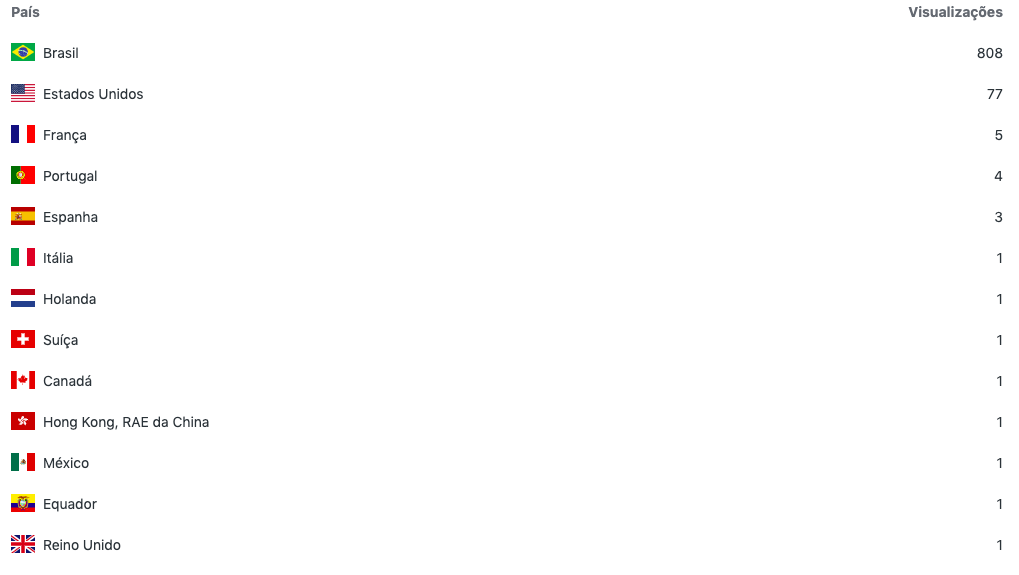
\includegraphics[width=1\textwidth]{Images/acessos-geo-cts-brasil.png}
    \caption{Acessos Geolocalizados ao CTS Brasil Blog.}
    \label{fig:acessos-geo-cts-brasil}
\end{figure}

Tendo em mente estes casos de sucessos na criação de conteúdos, que são de fato lidos pela sociedade além dos muros da universidade, decidimos que convidaríamos para participar das editatonas de nossa pesquisa as redes que orbitam o Laboratório de Informática e Sociedade (LabIS) da COPPE/UFRJ, fazendo com que nosso trabalho de campo tenha um efeito colateral um tanto quanto interessante: enquanto estudamos os mecanismo de governança da Wikipédia, criamos conteúdos livres em português sobre assuntos relacionados a Ciências-Tecnologias-Sociedades locais, tais como moedas sociais, softwares para acessibilidade, educação popular, informática e educação, mobilização política em redes sociais e demais assuntos que interessarem aos participantes das atividades. Promovemos assim maior acesso de leitores/as do idioma português, por todo o mundo, a esses conteúdos muitas vezes ignorados nos meios de divulgação científica e marginalizados por grande veículos de comunicação.

\subsection{Contar como foram nossas editatonas}